\documentclass{article}
\usepackage{amsmath}
\usepackage{amssymb}
\usepackage{graphicx}
\usepackage{hyperref}
\usepackage[version=4]{mhchem}


\begin{document}
\section*{Problem}
Show that if any two sides and the median on the third side of one triangle are equal to the corresponding sides and the median of the other triangle, the two triangles are congruent.

\section*{Solution}
As shown in the figure below, in \(\triangle A B C\) and \(\triangle A_{1} B_{1} C_{1}, A B=A_{1} B_{1}, A C=A_{1} C_{1}\), and \(A M=A_{1} M_{1}\).

Extend \(A M\) to \(N, A_{1} M_{1}\).to \(N_{1}\) such that \(A M=M N, A_{1} M_{1}=M_{1} N_{1}\), respectively.\\
\centering
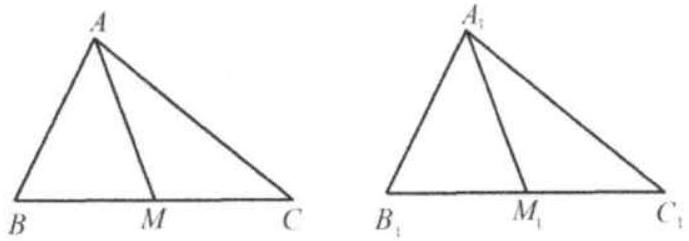
\includegraphics[width=\textwidth]{images/031.jpg}

Connect \(B N\) and \(B_{1} N_{1}\).\\
Since \(B M=M C, A M=M N, \angle A M C=\) \(\angle N M B, \triangle A M C \cong \triangle N M B\).

Similarly, \(\Delta A_{1} M_{1} C_{1} \cong \Delta N_{1} M_{1} B_{1}\).\\
Thus \(B N=A C=A_{1} C_{1}=B_{1} N_{1}\),\\
\centering
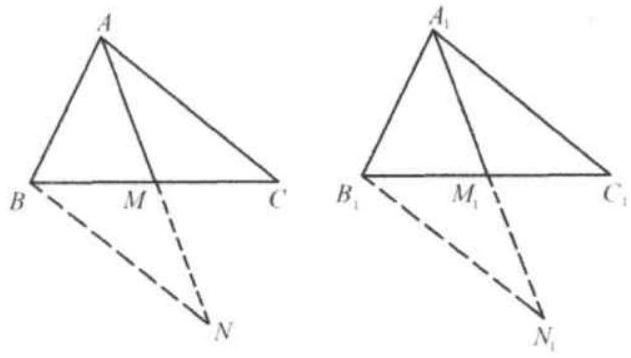
\includegraphics[width=\textwidth]{images/031(1).jpg}

In \(\triangle A B N\) and \(\triangle A_{1} B_{1} N_{1}, A B=A_{1} B_{1}, B N=B_{1} N_{1}\), and \(A N=A_{1} N_{1}\).\\
Thus \(\triangle A B N \cong \triangle A_{1} B_{1} N_{1}\).

Draw a line connecting the midpoints of triangle or trapezoid.
Theorem 2.1. The line segment whose endpoints are the midpoints of two sides of a triangle is parallel to the third side of the triangle and has a measure equal to one-half of the measure of the third side.\\
\(M N / / B C\).\\
\(M N=\frac{1}{2} B C\)\\
\centering
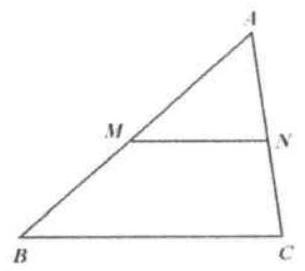
\includegraphics[width=\textwidth]{images/032(2).jpg}\\
\(M N\) is called the midline of \(\triangle A B C\).

Proof:
Let \(M, N\) be the midpoints of \(A B\) and \(A C\), respectively. Connect \(B N\) and \(C M\).\\
Since \(M\) is the midpoints of \(A B, S_{\triangle C B M}=\frac{1}{2} S_{\triangle A B C}\).\\
\centering
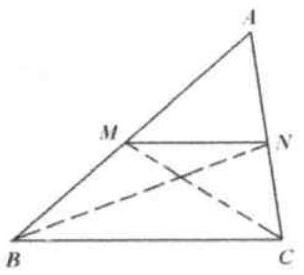
\includegraphics[width=\textwidth]{images/032.jpg}

Since \(N\) is the midpoints of \(A C, S_{\triangle B C N}=\frac{1}{2} S_{\triangle A B C}\).\\
\centering
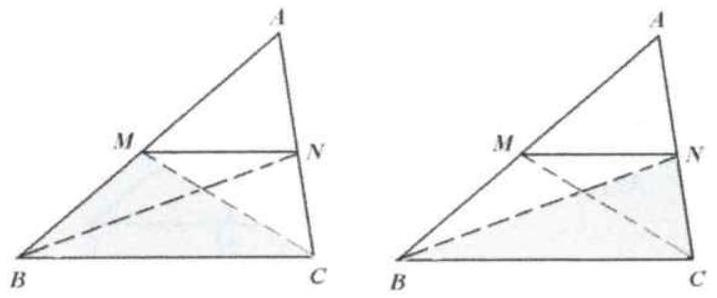
\includegraphics[width=\textwidth]{images/032(1).jpg}

So \(S_{\triangle C B M}=S_{\triangle B C N}\)\\
Thus \(M N / / B C\).\\
\(\frac{S_{\triangle N M B}}{S_{\triangle B N C}}=\frac{\frac{1}{2} M N \times B N}{\frac{1}{2} B C \times B N}=\frac{M N}{B C}\)

\section*{Chapter 2 Draw the Auxiliary Lines with the Midlines}
\begin{center}
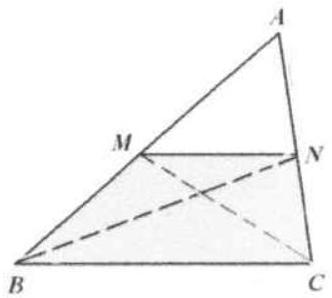
\includegraphics[width=\textwidth]{images/033.jpg}
\end{center}

We see from the figures below that\\
\(S_{\triangle N M B}=S_{\triangle A M N}=\frac{1}{4} S_{\triangle A B C}\)\\
\(S_{\triangle B N C}=S_{\triangle B N A}=\frac{1}{2} S_{\triangle A B C}\)\\
Substituting (2) and (3) into (1):\\
\(\frac{\frac{1}{4} S_{\triangle A B C}}{\frac{1}{2} S_{\triangle A B C}}=\frac{M N}{B C} \quad \Rightarrow \quad \frac{1}{2}=\frac{M N}{B C} \quad \Rightarrow M N=\frac{1}{2} B C\).\\
\centering
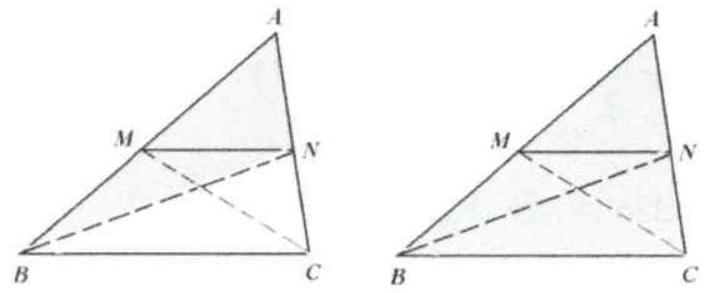
\includegraphics[width=\textwidth]{images/033(2).jpg}

Theorem 2.2. If a line contains the midpoint of one side of a triangle \((A B)\) and is parallel to a second side \((A C)\) of the triangle, then it will bisect the third side of the triangle.\\
\(A N=N C\).

Proof:
Let \(M\) be the midpoint of \(A B\) and \(A M N / / B C\).\\
\centering
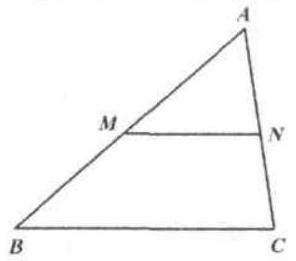
\includegraphics[width=\textwidth]{images/033(1).jpg}

Connect \(B N\) and \(C M\).\\
\(\triangle A M N \sim \triangle A B C\).


Thus \(\frac{A M}{A N}=\frac{M B}{N C} \quad \Rightarrow \quad \frac{\frac{1}{2} A B}{A N}=\frac{\frac{1}{2} A B}{N C} \Rightarrow \quad A N=N C\).

Theorem 2.3. For any trapezoid \(A B C D\), the following relationship is true:\\
\(M N=\frac{1}{2}(A D+B C)\)\\
\(M\) and \(N\) are the midpoints of \(A B\) and \(B C\), respectively. \(M N\) is the median of the trtapezoid.\\
\centering
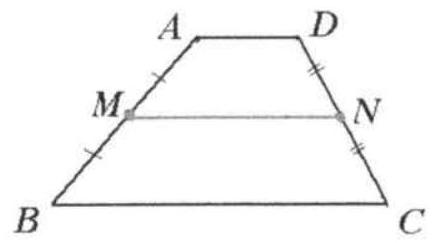
\includegraphics[width=\textwidth]{images/034(1).jpg}

Proof:
Connect \(D B\) and \(D B\) meets \(M N\) at \(E\).\\
In triangle \(B C D\), since \(M N / / B C, E N / / B C\).\\
By Theorem 2.2, \(E\) is the midpoint of \(B D\).\\
\centering
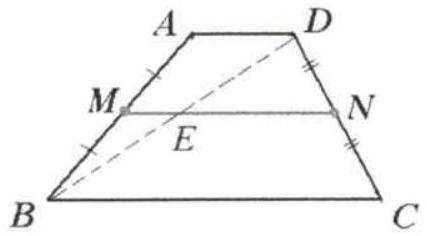
\includegraphics[width=\textwidth]{images/034(2).jpg}

By Theorem 2.1, \(E N=\frac{1}{2} B C\)\\
In triangle \(A D B\), since \(M N / / A D, M E / / A D\).\\
By Theorem 2.2, \(E\) is the midpoint of \(B D\).\\
By Theorem 2.1, \(M E=\frac{1}{2} A D\)\\
(2) \(+(1): M N=\frac{1}{2}(A D+B C)\)

Theorem 2.4. For any trapezoid \(A B C D\), the following relationship is true:\\
\(M N=\frac{1}{2}(B C-A D)\)\\
\centering
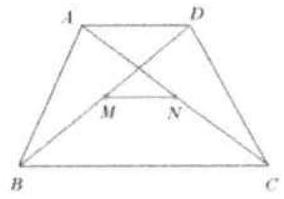
\includegraphics[width=\textwidth]{images/034.jpg}


\(M\) and \(N\) are the midpoints of the diagonals \(A C\) and \(B D\), respectively.

Proof:
Connect \(D N\) and extend \(D N\) to meet \(B C\) at \(E\).\\
Since \(A D / / B C, \angle D A N=\angle E C N, \angle A D N=\angle C E N\), and \(A N=N C\),\\
Thus \(\triangle A D N \cong \triangle E C N, D N=N E, A D=C E\).\\
\centering
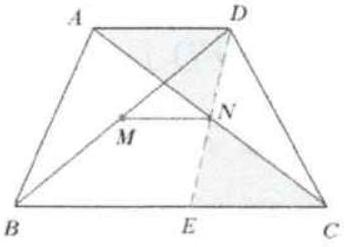
\includegraphics[width=\textwidth]{images/035(3).jpg}

We also know that \(D M=M B\).

By Theorem 2.1, we have \(M N / / B E\) and\\
\(M N=\frac{1}{2} B E=\frac{1}{2}(B C-C E)=\frac{1}{2}(B C-A D)\)\\

\end{document}
